\documentclass{anstrans}
%%%%%%%%%%%%%%%%%%%%%%%%%%%%%%%%%%%
\title{An Improved ANS Transaction Template}
\author{Baptiste Mouginot,$^{*}$ Kathryn Mummah,$^{*}$ Paul P.H. Wilson$^{*}$}

\institute{
$^{*}$University of Wisconsin-Madison, WI
}

\email{mouginot@wisc.edu \and mummah@wisc.edu \and paul.wilson@wisc.edu}

% Optional disclaimer: remove this command to hide
% \disclaimer{Notice: this manuscript is a work of fiction. Any resemblance to
% actual articles, living or dead, is purely coincidental.}

%%%% packages and definitions (optional)
\usepackage{graphicx} % allows inclusion of graphics
\usepackage{booktabs} % nice rules (thick lines) for tables
\usepackage{microtype} % improves typography for PDF
\usepackage{float}

\newcommand{\SN}{S$_N$}
\renewcommand{\vec}[1]{\bm{#1}} %vector is bold italic
\newcommand{\vd}{\bm{\cdot}} % slightly bold vector dot
\newcommand{\grad}{\vec{\nabla}} % gradient
\newcommand{\ud}{\mathop{}\!\mathrm{d}} % upright derivative symbol

\begin{document}
%%%%%%%%%%%%%%%%%%%%%%%%%%%%%%%%%%%%%%%%%%%%%%%%%%%%%%%%%%%%%%%%%%%%%%%%%%%%%%%%
\section{Introduction}




Some text for introduction etc\ldots
Some text for introduction etc\ldots
Some text for introduction etc\ldots
Some text for introduction etc\ldots
Some text for introduction etc\ldots
Some text for introduction etc\ldots
Some text for introduction etc\ldots
Some text for introduction etc\ldots
Some text for introduction etc\ldots
Some text for introduction etc\ldots
Some text for introduction etc\ldots
Some text for introduction etc\ldots
Some text for introduction etc\ldots
Some text for introduction etc\ldots
Some text for introduction etc\ldots
Some text for introduction etc\ldots
Some text for introduction etc\ldots
Some text for introduction etc\ldots
Some text for introduction etc\ldots
Some text for introduction etc\ldots
Some text for introduction etc\ldots
Some text for introduction etc\ldots
Some text for introduction etc\ldots
Some text for introduction etc\ldots


%%%%%%%%%%%%%%%%%%%%%%%%%%%%%%%%%%%%%%%%%%%%%%%%%%%%%%%%%%%%%%%%%%%%%%%%%%%%%%%%
\section{Theory}



Some text for introduction etc\ldots
Some text for introduction etc\ldots
Some text for introduction etc\ldots
Some text for introduction etc\ldots
Some text for introduction etc\ldots
Some text for introduction etc\ldots
Some text for introduction etc\ldots
Some text for introduction etc\ldots
Some text for introduction etc\ldots
Some text for introduction etc\ldots
Some text for introduction etc\ldots
Some text for introduction etc\ldots
Some text for introduction etc\ldots
Some text for introduction etc\ldots
Some text for introduction etc\ldots
Some text for introduction etc\ldots


\section{Cascade Enrich Construction}
\subsection{Centrifuge properties}
The present work uses the analytical solution by R\"aetz \cite{ref} of the
differential equation for the gas centrifuge as described in \cite{Glaser2008}. Centrifuge parameters, such as average gas temperature, rotation speed, height, feed flow rate, diameter, pressure ratio,
counter-current flow ratio, and efficiency have been chosen to match the cascade design
describe in \cite{glaser2008} and \cite{Walker2017}. These parameters for a P1-type centrifuge are used to estimate the Joint Comprehensive Plan of Action (JCPOA)-compliant IR-1 centrifuge.


\subsection{Cascade Design}

The cascade is built to be ideal, defined by $\alpha =\beta = const$
for all stage of the cascade, where $\alpha$ and $\beta$ respectively represent
the feed to product and the feed to tail enrichment factors.
$\alpha$ can be expressed as a function of the feed rate $F$, the separative performance $\delta U(\theta)$ and $\theta$,
and $\beta$ as a function of $alpha$ and $\theta$:
\begin{subequations} \label{eqs:alphabeta}
    \begin{equation} \label{eq:alpha}
    \alpha = \sqrt{\frac{2\delta U}{F} \frac{1-\theta}{\theta}}+1
\end{equation}
\\
\begin{equation}\label{eq:beta}
    \beta = R
              \dfrac{1 - \dfrac{N - \theta \dfrac{\alpha R}{1+\alpha R}}{1 - \theta}}
                   {\dfrac{N - \theta \dfrac{\alpha R}{1+\alpha R}}{1 - \theta}}
\end{equation}
\end{subequations}

From equation \eqref{eq:alpha} and \eqref{eq:beta} it is possible to determine the cut, or the ratio of product flow to feed flow.
%(all other centrifuge parameters been fixed) allowing the have $\alpha=\beta$
required to build an ideal cascade.

Since $\alpha_{i}$ and $\beta_{i}$ remain constant, only the value of the cut, $\theta_{i}$, changes in each stage of a cascade.

It can be shown that $\theta_{i}$ can be computed from $\alpha$,
$\beta$ values and the feed assay, $N_{i}$ \cite{ref}:
\begin{eqnarray}
    \theta_{i} &=& \dfrac{N_{i} - N''_{i}}{N'_{i}-N''_{i}}\nonumber\\
           &=& \dfrac{N_{i} - \dfrac{1}{1 + \beta/R_{i}}}{ \dfrac{\alpha R_{i}}{1 + \alpha R_{i}} -
           \dfrac{1}{1 + \beta/R_{i}}}
\end{eqnarray}

This algorithm assumes that the corresponding separative power $\delta U$ (not re-computed) can be
achieved with the chosen centrifuge design. Once $\theta_{i}$ determined, it is possible to
compute the product and the tail assay.

The design of the cascade is performed through 2 steps. First one determines the
configuration and number of stages, adding stages following the previously
described procedure, until $N'_{last} > N'_{requested}$ and $N''_{last} <
N''_{requested}$. (Note that $N'_{last}$ corresponds to the product assay of the
last enrichment stage, and $N''_{last}$ to the tail assay of the last stripping
stage). This allows to determine the number of enriching and stripping stages as
well as their enrichment properties ($N_{i}$, $N'_{i}$,
$N''_{i}$,$\theta_{i}$i).
% might be more useful to the reader to say this in words instead of variables, i.e. adding stages until the product assay of the final stage is greater than or equal to than the desired assay, and the tails assay is similarly less than or equal to the desired tails assay

The second step determines how to populate the cascade with the user-defined maximum number of centrifuges. One first solves the linear flow equation to determine the theoretical flow in the
cascade:
\begin{strip}
\begin{equation}
\setcounter{MaxMatrixCols}{20}
\begin{bmatrix}
-1         & 1-\theta_{S+1} & 0              & 0 & ... & 0 & 0            & 0   & 0              & 0 & ... & 0            & 0            & 0 \\
\theta_{S} & -1             & 1-\theta_{S+2} & 0 & ... & 0 & 0            & 0   & 0              & 0 & ... & 0            & 0            & 0 \\
           &                &                &   &     &   &              & ... &                &   &     &              &              &   \\
0          & 0              & 0              & 0 & ... & 0 & \theta_{-1}  & -1  & 1 - \theta_{1} & 0 & ... & 0            & 0            & 0 \\
           &                &                &   &     &   &              & ... &                &   &     &              &              &   \\
0          & 0              & 0              & 0 & ... & 0 & 0            & 0   & 0              & 0 & ... & \theta_{E-2} & -1           & 1-\theta_{E} \\
0          & 0              & 0              & 0 & ... & 0 & 0            & 0   & 0              & 0 & ... & 0            & \theta_{E-1} & -1
\end{bmatrix}
\times
\begin{bmatrix}
     F_{S}   \\
     F_{S+1} \\
     \cdots  \\
     F_{0}   \\
    \cdots   \\
    F_{E-1}  \\
    F_{E}
\end{bmatrix}
=
\begin{bmatrix}
     0   \\
     0 \\
     \cdots  \\
     F   \\
    \cdots   \\
    0  \\
    0
\end{bmatrix}
%\caption{caption needed!}
\label{eq:flow}
\end{equation}
\end{strip}
Once the relative flow of each stage, $F_{i}$, has been determined, the
cascade can be populated with actual machines up the stages
until either the maximum number available of machines or the maximum feed
flow is reached.


\subsection{Response to an non-ideal feed - $\theta_{i} = const$ hypothesis}

Little information is available about the optimum way to tune a cascade that is being fed a feed enrichment that does not match its ideal enrichment.

The tuning method outlined here does not re-optimize $\theta_i$ based on the true flow enrichment. As $\delta
U$ and $\alpha$ do not depend on the stage feed assay $N'$ and the feed to product
ratio $\alpha$ do not change from stage to stage. According to equation
\eqref{eq:beta}, when $\alpha$ and $\theta$ are fixed, if the feed assay,
$N$ changes, then $\beta$ will change accordingly.  This brakes the
ideal status of the cascade, i.e.  $N_{i} \neq N'_{i-1} \neq N''_{i+1}$.

In order to compute the proper product and tails assay at each stages\, the tails and the product from respectively the next and the
previous stage must be blended in order to determine the correct stage feed assay. As this is a
obvious cycling problem, it has been chosen to solve it iteratively: all feed
assay are iteratively updated, blending the proper product and tail, then using
the updated feed assay, the new product and tail assay are recomputed. This
process is repeated until the change in assays is smaller than the
set precision (1e-8 by default).

Other hypotheses will be explored in the future, such as maintaining the ideal
stage of the cascade through tuning the cut values $\theta_{i}$ of each
stage of the cascade, or maintaining $\alpha*\beta = const$ as described in
\cite{walker2017}.

Note that as a consequence of our design method, the cascade product and tail
assay will not necessary match the targeted values, and usually slightly over
enrich and over strip the product and the tail respectively.

\section{The experiment}

As explained previously, the goal of this work is to assess the rate of the highly-enriched uranium (HEU)
production using enrichment cascades designed within the JCPOA agreement
constraints. For this work, two different cases will be investigated and compared
to the reference case.

All cases will be considered with and without tail recycling. Figure
\ref{fig:flow} shows the different flows between the different facilities in the
fleet, in a configuration with two different levels of cascade without tail
recycling. When considering the tail recycling, all the flow going from a
cascade to the waste, are going from the cascade $i$ to the cascade $i-1$.
The Storage are not required in Cyclus they have been added to ensure the
proper material flow between the facilities (if a receiver facility input buffer
is full then the sender facility will stop sending material to it, and will stop
working when its own output buffer will be filled).

\begin{figure}[ht] % replace 't' with 'b' to force it to be on the bottom
  \centering
  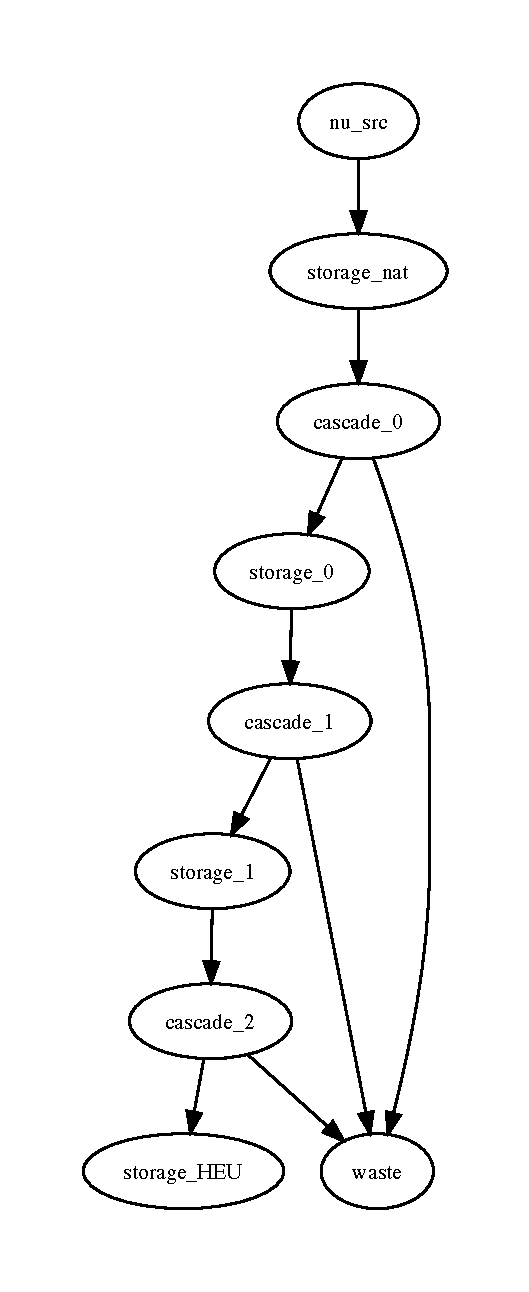
\includegraphics[scale=0.7]{flow_case_2_no_recy.pdf}
  \caption{Illustration of the material flow between the different level of
      cascades without tail recycling, in this diagram, nu\_src correspond to an
      infinite source of natural uranium, cascade\_ $n$ and storage\_ $n$
      corresponds respectively to the cascades, and the storage getting the
  products of the cascades at the level $n$.}\label{fig:flow}
\end{figure}

\subsection{Explored Cases}
\subsubsection{Reference Case}
The reference case corresponds to the most ideal cascade design--utilizing all of the 5060
centrifuges available within JCPOA to produce an enriched product at $>90\%$ of U-235,
stripping the tail product up to 0.28 $\%$ from a feed of natural uranium.
The design cascade in this case, includes 4 stripping stages, and 38 enriching
stages. The Feed/Product/Tail (F/P/T) assays are respectively
0.0071/0.903/0.0028.
%maybe include some cascade shape figures?

\subsubsection{Case 1}
The case 1 is designed to configure 30 cascades in the scenario (the maximum allowable under
the JCPOA agreement), all designed the same way. The basic properties are:\\
- less than 169 centrifuges per cascade,\\
- F/P/T assays: 0.0071/0.035/0.003.\\
The corresponding design is:\\
- 167 centrifuges,\\
- F/P/T assays: 0.0071/0.0412842/0.00290548.\\

\subsubsection{Case 2} Case 2 also limited to 30 cascades in the scenario (the
maximum allowable under the JCPOA agreement), but this time each level of
cascades are designed to take feed from the previous level's product. Each
cascade has 4 stripping stages and 10 enriching stages. The configuration of
cascade levels can be found in table \ref{tab:cascadelvl}. Unlike case 1, the
organization of centrifuges varies from level to level. Each level is re-optimized
to have the most efficient number of centrifuges in each stage, although the total number
of stages remains constant. T

 %we haven't defined a level

\begin{table}[htb]
\centering
\begin{tabular}{cllll}
\toprule

Level   &           & Assay     &       & Machines  \\
        & Feed      & Product   & Feed  &           \\
\midrule
0       & 0.0071    & 0.0413    & 0.0029 & 167       \\
1       & 0.0413    & 0.2043    & 0.0173 & 169       \\
2       & 0.2043    & 0.5941    & 0.0971 & 168       \\
3       & 0.5941    & 0.8834    & 0.3915 & 168       \\
4       & 0.8834    & 0.9735    & 0.7746 & 169       \\

\bottomrule
\end{tabular}
  \caption{Summary of cascade properties for each level}
  \label{tab:cascadelvl}
\end{table}


\subsection{Level optimization}
A last round of optimization if then ran in order to limit the number of cascade
level to the amount of level required produce HEU, and then to populate the
different level with a total of 30 cascades in order to maximize the HEU
production rate.

\section{Results}
\subsection{Enrichment}
\subsubsection{Without tail recycling}
Despite the reconfiguration of each level occurring in the second case, the case
1 is notably more effective in producing HEU than case 1. Indeed, as observed in Figure
\ref{fig:assay_c1_rc} and \ref{fig:assay_c2_rc}, the first case is able to
produce an uranium product enrich at $98\%$ while the second case is only able
to reach an enrichment of $88.3\%$ with the same number of levels.

\begin{figure}[ht] % replace 't' with 'b' to force it to be on the bottom
  \centering
  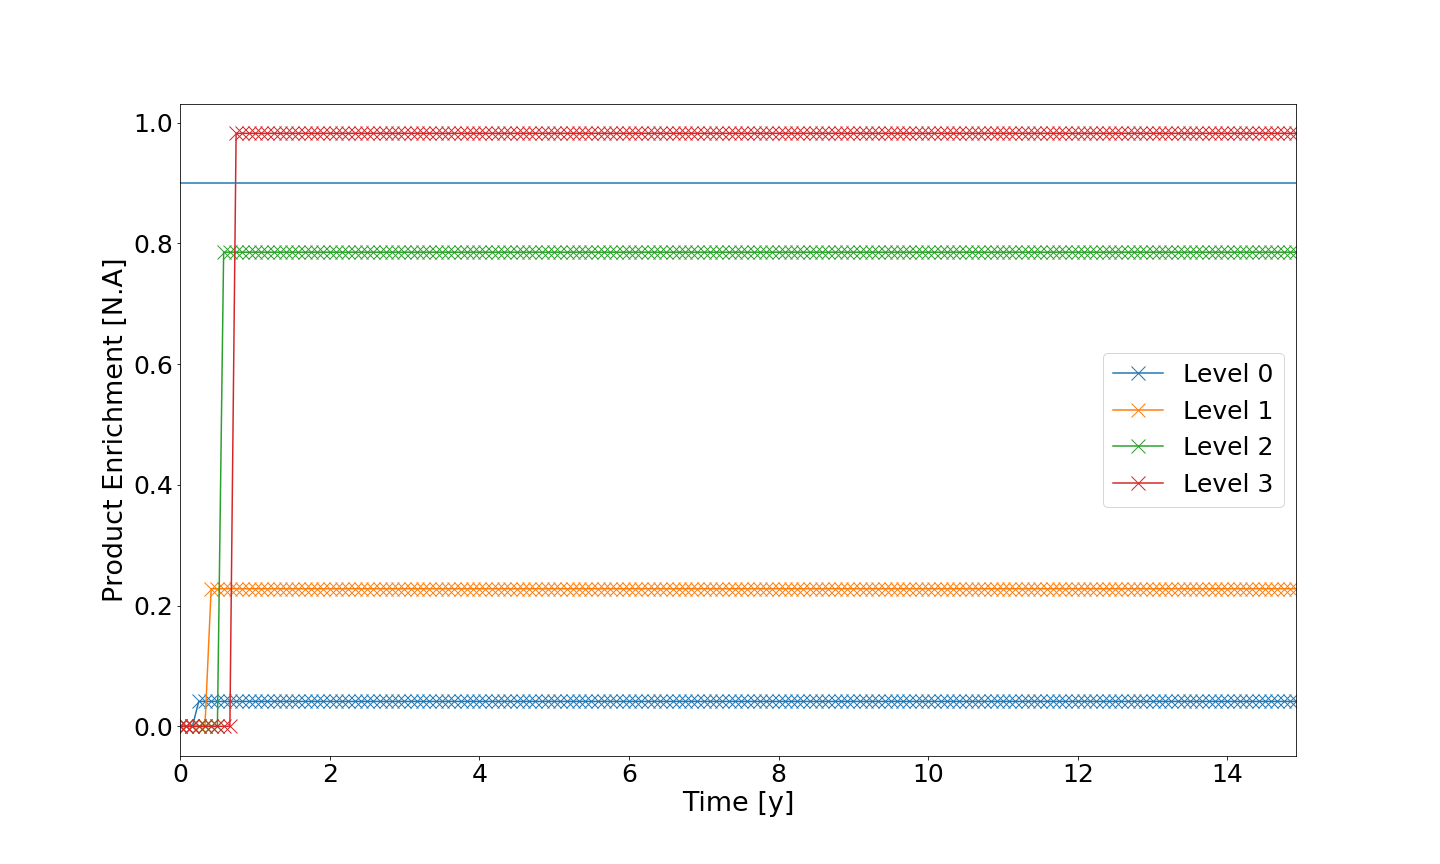
\includegraphics[width=0.5\textwidth]{assay_case_1_no_rec.png}
  \caption{Evolution of the different product assays at each cascade level for
  the case 1 without recycling. The blue line represents the $90\%$ enrichment
  threshold.}\label{fig:assay_c1_nr}
\end{figure}
\begin{figure}[ht] % replace 't' with 'b' to force it to be on the bottom
  \centering
  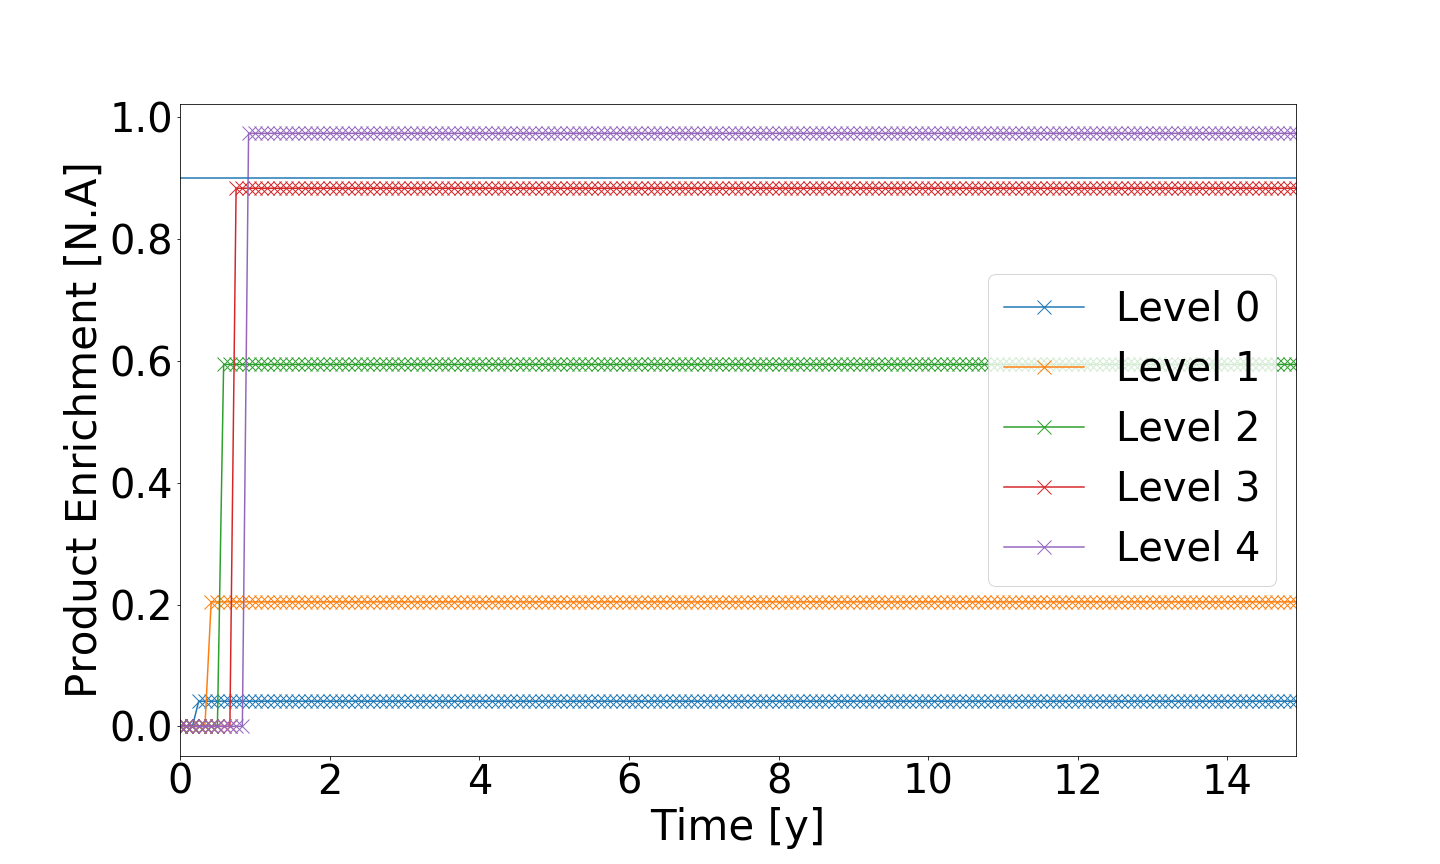
\includegraphics[width=0.5\textwidth]{assay_case_2_no_rec.png}
  \caption{Evolution of the different product assays at each cascade level for
  the case 2 without recycling. The blue line represents the $90\%$ enrichment
  threshold.}\label{fig:assay_c2_nr}
\end{figure}

Because the cut value $\theta_i$ at each stage is unchanged, case 2 artificially
produces over-enriched tails when fed with higher enriched materials compared
to a cascade feed with the same feed assay but with a cascade designed for it.

% ^ the above paragraph is confusing but I don't understand it enough to fix it

The effective cut values for each cascade can be computed as :

\begin{equation}\label{eq:theta_eff}
    \theta = \dfrac{N - N''}{N'-N''}
\end{equation}

\begin{table}[htb]
\centering
\begin{tabular}{cll}
\toprule

Level   &  $\theta_{eff}^{C1}$   & $\theta_{eff}^{C2}$ \\
\midrule
1       & 0.109375               & 0.109375     \\
2       & 0.109375               & 0.128342     \\
3       & 0.109375               & 0.215694     \\
4       & 0.109375               & 0.411872     \\
5       & 0.109375               & 0.547009     \\

\bottomrule
\end{tabular}
  \caption{Cascade effective $\theta$ by the level and case.}
  \label{tab:cascade_theta}
\end{table}
As illustrated in Table \ref{tab:cascade_theta}, the effective cut
of each level increases up to $0.54$ for the fifth stage for case 2. The high
effective cut value increase the product production rate but decrease the
enrichment ratio.

\subsubsection{tails recycling}
When recycling the tails from the different cascade levels, both cases behave
the same way. As the tails have an higher enrichment than the product then are
blended to, recycling the tail has the effect to bump up the enrichment of the
product at each level (see Figure \ref{fig:assay_c1_r} and \ref{fig:assay_c2_r}).

\begin{figure}[ht] % replace 't' with 'b' to force it to be on the bottom
  \centering
  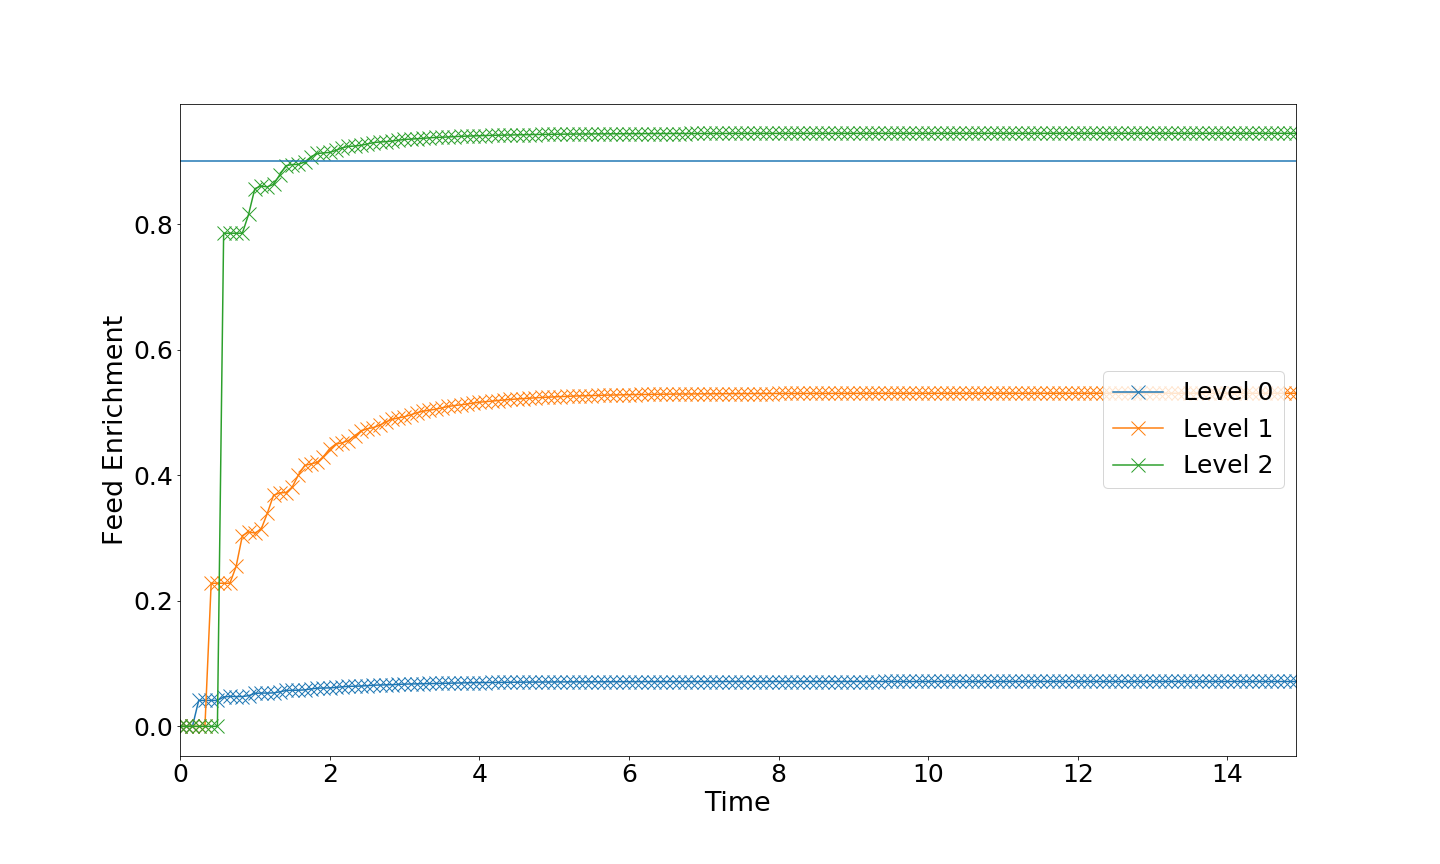
\includegraphics[width=0.5\textwidth]{assay_case_1_rec.png}
  \caption{Evolution of the different product assays at each cascade level for
  the case 1 with recycling. The blue line represents the $90\%$ enrichment
  threshold.}\label{fig:assay_c1_r}
\end{figure}

Note that for the case 2, where the fourth stage could appear as useless only the
blending of its tail allows the product of the third one to pass the $90\%$ threshold.

\begin{figure}[ht] % replace 't' with 'b' to force it to be on the bottom
  \centering
  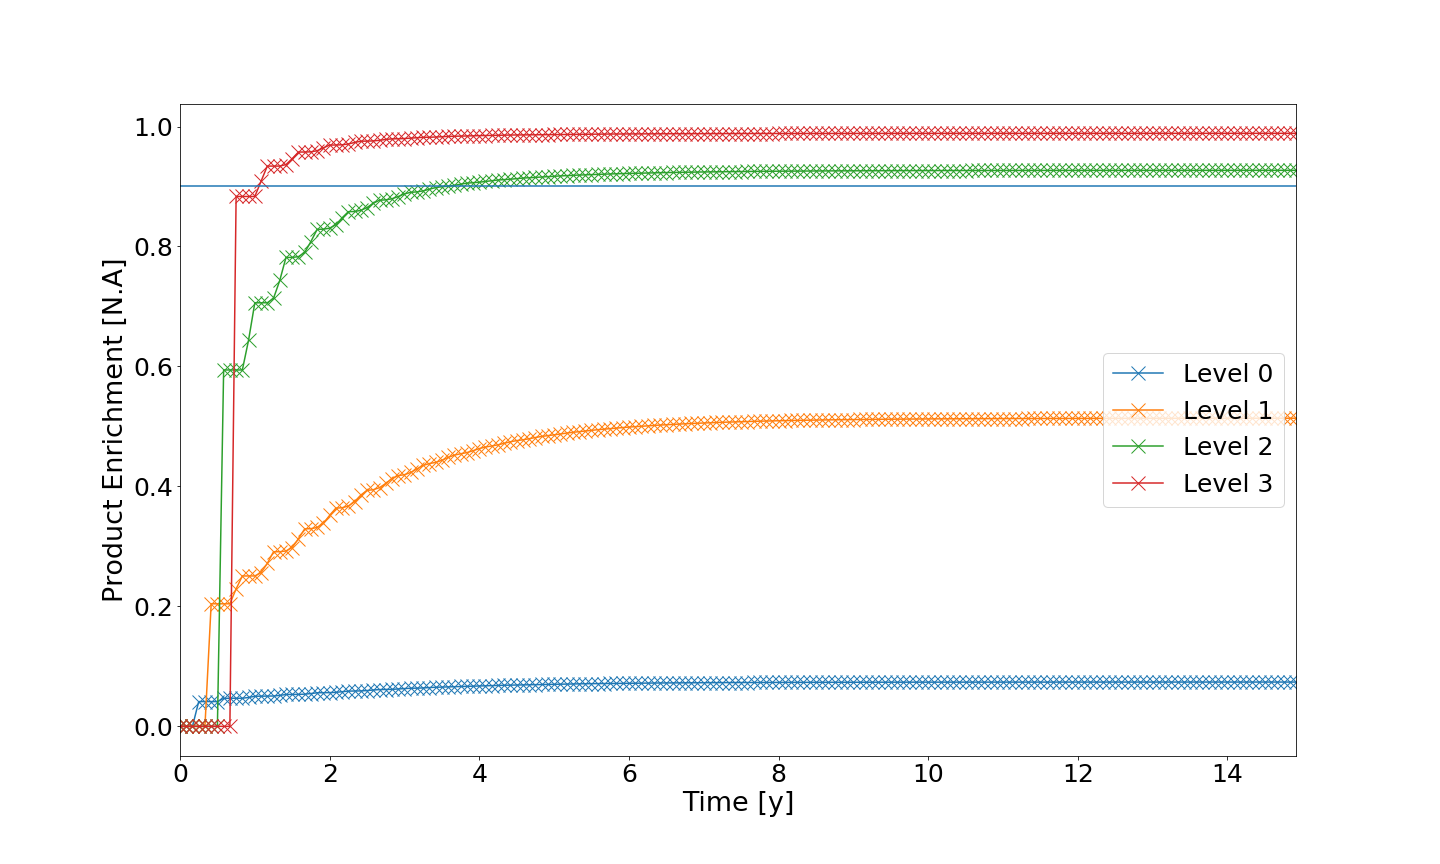
\includegraphics[width=0.5\textwidth]{assay_case_2_rec.png}
  \caption{Evolution of the different product assays at each cascade level for
  the case 2 with recycling. The blue line represents the $90\%$ enrichment
  threshold.}\label{fig:assay_c2_r}
\end{figure}


\subsection{HEU flow rate}
As shown Figure \ref{fig:heu_prod}, if using all the centrifuges available to
build a big cascade dedicated to HEU production, only 8 months are required to
produce 1 Significant Quantity (SQ) of HEU. Also it take significantly longer to
build 1 SQ of HEU, without recycling the tails respectively 13 years and 3.5 year
for the case 1 and 2 versus about 2 years with tail recycling.

\begin{figure}[ht] % replace 't' with 'b' to force it to be on the bottom
  \centering
  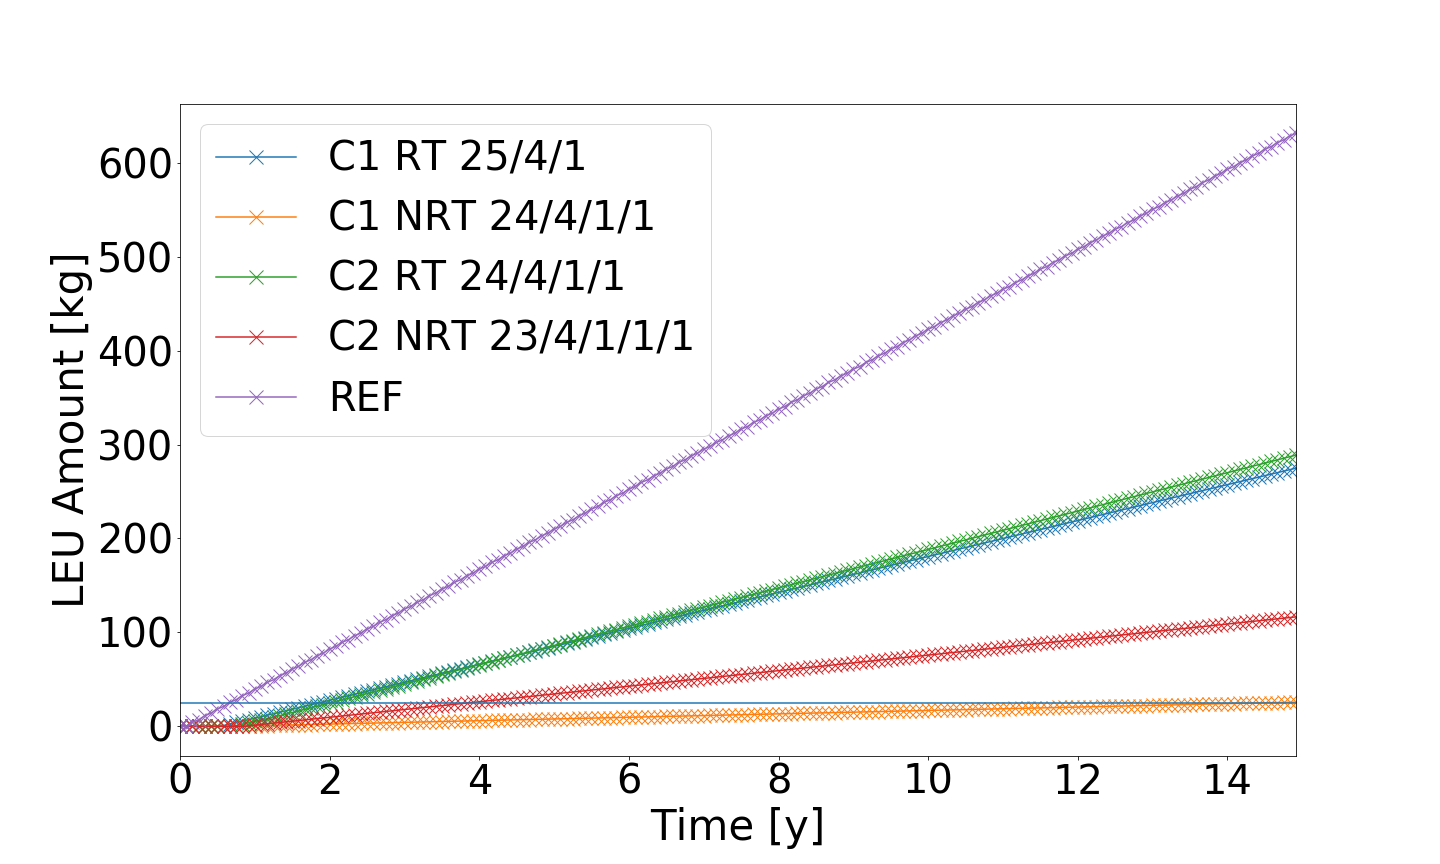
\includegraphics[width=0.5\textwidth]{HEU_prod.png}
  \caption{Evolution of the amount of HEU in the storage. The blue line
  correspond to one significant quantity of HEU ($25~$kg). CX correpsonds to the
  case number(1 or 2), RT and NRT the tail reprocessing or not ones. W/X/Y/Z represent the
  number of cascade per level. REF corresponds to the reference
  case.}\label{fig:heu_prod}
\end{figure}

It is also interresting to note that despite requiering more level of cascade to
reach an enrichment of $90\%$ the second case with tial recycling produces HEU
at a equivalent rate than the case 1. The production rate seems to be faster but
require more time to reach the maximum production rate (the material have to
flow through more levels to reach the final level).

%%%%%%%%%%%%%%%%%%%%%%%%%%%%%%%%%%%%%%%%%%%%%%%%%%%%%%%%%%%%%%%%%%%%%%%%%%%%%%%%
%%%%%%%%%%%%%%%%%%%%%%%%%%%%%%%%%%%%%%%%%%%%%%%%%%%%%%%%%%%%%%%%%%%%%%%%%%%%%%%%
\section{Conclusions}

The included ANS style file and this clear example file are a panacea for
the hours of headache that invariably results from formatting a document in
Microsoft Word.

%%%%%%%%%%%%%%%%%%%%%%%%%%%%%%%%%%%%%%%%%%%%%%%%%%%%%%%%%%%%%%%%%%%%%%%%%%%%%%%%
\appendix
\section{Appendix}

Numbering in the appendix is different:
\begin{equation} \label{eq:appendix}
  2 + 2 = 5\,.
\end{equation}
and another equation:
\begin{equation} \label{eq:appendix2}
  a + b = c\,.
\end{equation}

%%%%%%%%%%%%%%%%%%%%%%%%%%%%%%%%%%%%%%%%%%%%%%%%%%%%%%%%%%%%%%%%%%%%%%%%%%%%%%%%
\section{Nomenclature}

\begin{table}[H]
    \centering
    \begin{tabular}{l|l}
%         &  \\
        $N$ & Feed assay \\
        $N'$ & Product assay \\
        $N''$ & Tails assay \\
        $\alpha$ & Feed to product enrichment factor \\
        $\beta$ & Feed to tail enrichment factor \\
        $\theta$ & Cut
    \end{tabular}
%    \caption{Caption}
    \label{tab:my_label}
\end{table}

%%%%%%%%%%%%%%%%%%%%%%%%%%%%%%%%%%%%%%%%%%%%%%%%%%%%%%%%%%%%%%%%%%%%%%%%%%%%%%%%
\section{Acknowledgments}
This material is based upon work supported a Department of Energy Nuclear
Energy University Programs Graduate Fellowship.

%%%%%%%%%%%%%%%%%%%%%%%%%%%%%%%%%%%%%%%%%%%%%%%%%%%%%%%%%%%%%%%%%%%%%%%%%%%%%%%%
\bibliographystyle{ans}
\bibliography{bibliography}
\end{document}
